\documentclass[11pt,a4paper]{article}

\usepackage[english]{babel}
\usepackage[T1]{fontenc}
\usepackage[utf8]{inputenc}
\usepackage{graphicx}
\graphicspath{ {files/}}
\usepackage[usenames, dvipsnames]{color}
\usepackage{url}

\title{Separation of Concerns: 
You need it! Here is why.}
\author{Joy van den Eijkhof}
\date{04/11/2017}


\begin{document}
\maketitle
\noindent
\begin{abstract}
One of the most fundamental design principles in Computer Science and programing is Separation of Concerns (SoC). It is the means to keep order and structure, as well as flexibility within code. It is important, yet not always easy to grasp for the inexperienced programmer. Therefore, this essay is for the beginner, by a beginner, to discuss the purpose, the importance as well as the benefits of applying SoC to programming.\linebreak  \linebreak \linebreak
\end{abstract}

\begin{center}
 This essay is an attempt to reach IOOPM goals K32 and X59
\end{center}

\pagebreak
\maketitle
\begin{flushleft}
\section{Introduction}
How can one eat an elephant? One bite at a time. How does one tackle a big problem? One small problem at a time. The principle of Separation of Concerns (SoC) deals with the dividing of a problem, in this case the elephant, into manageable pieces. More formally, SoC states that each element of a larger complex should have one coherent purpose, and have as little overlapping as possible with the other elements.\footnote{Makabee, Hayim. “Separation of Concerns.” \textit{Effective Software Design}, 5 Feb. 2012, effectivesoftwaredesign.com/2012/02/05/separation-of-concerns/.} In programming, high SoC can be achieved through modularity and encapsulating concerns. In contrast very low SoC could be having all code regarding one program in one main function. At first it might seem attractive to have all code in one place, but for it to be easier to write, develop and maintain, SoC is an invaluable principle to follow.

\section{The Purpose}

The purpose of SoC is to create order from the complex. This order, in turn, makes programming more manageable and feasible. In the programming language C this can be achieved by writing code in separate coherent modules with low coupling; by for example, separating one module that handles the logic behind linked lists from the logic of binary trees. It is important to note that low coupling should not be sacrificed for high coherency, or in other words, each function should not be its own module. This would defeat the purpose of order. It is the order that is the reason SoC is so effective, for it enables a more programmer friendly code-environment.
\section{The Importance}
SoC is worth it. Its benefits are both in time, head space and in some instances even financial. The main benefits can be boiled down to this: Code is easier to handle when one only needs to deal with one piece of it at a time, and one can do that. To the developer SoC allows for the solving of one problem at a time in an orderly manner that helps create head space to solve the issue at hand, rather than being overwhelmed by the problem as a whole. It also makes it easier to reuse code, when it is encapsulated and has a singular purpose. To the one who needs to maintain the code, a change in one module las a low risk of breaking the rest of the program, when that module has low coupling with other modules, for example. Overall there are many benefits to SoC and it is worth the time and energy it takes to apply it to the program, or problem at hand.

\section{Implementing SoC}

Not applying SoC from the beginning can have a heavy cost. It goes without question that it is easier to structure a program and code from the beginning, rather than than try to untangle concerns after the fact. Consider for example the following piece of Java code: 

\begin{figure}[h!]
  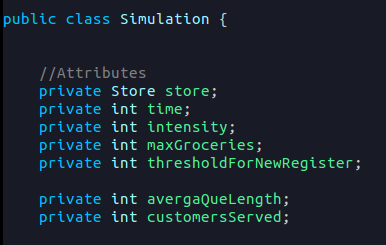
\includegraphics[width=15cm,height=6cm,keepaspectratio,]{Images/simulation}
  \caption{Simulation class}
  \label{Figure 1.1}
\end{figure}

In Figure 1 avergaQueLength and customersServed were attributes of the class Simulation. These existed for the purpose of being displayed as the statistics of the Simulation while it was running. At the time this code was first written, it seemed like enough. Soon however, there were more statistical information that needed to be displayed.  The choice was to either create a subclass called statistics, or add more attributes to the simulation class. Regardless, this change would affect other programs that relied on this class, this is therefore a concern, that could have benefitted from being its own class or subclass, from the beginning. In the example above, by trying to solve too many problems within one class, it created extra challenges later for the program developer who had to go back and change it. On a larger scale, in the business world, such a flaw could translate into financial cost. It pays of to do the work now by applying SoC early on, rather than paying a potential heavy price later on.

\section{The benefits}
Code that has been written according to the principles of SoC are ideally flexible and easily changed. In its very nature, such code should have few repetitions, modules and classes should have high coherency and low coupling. This in turn means that it should be easier to change underlying logic of a function, or add new aspects to a class without breaking the parts of the program that rely on these lines of code. Consider the following class in Java:     \linebreak

\begin{figure}[h!]
  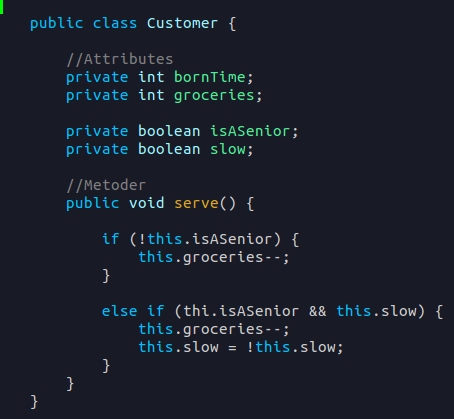
\includegraphics[width=18cm,height=6cm,keepaspectratio,]{Images/FulSenior.png}
  \caption{Customer class}
  \label{Figure 1.2}
\end{figure}

In Figure 2\footnote{van den Eijkhof, Joy E, and Ulf Sigvardsson. 2 Nov. 2017. Came up with the logic behind Serve().} the class Customer has the boolean attribute isASenior, and the method serve() acts differently depending upon weather isASenior is true or not. In short there are multiple things being handled within one class, and within one method. Consider if a third attribute was to be included, such as isAFamily, and serve() handled those with that attribute as true, differently from isASenior. There are suddenly multiple pieces of code that needs to be edited, and depending upon where else this class is used, that code needs editing too. Alternatively we can apply SoC to this problem:\linebreak \linebreak \linebreak \linebreak \linebreak \linebreak \linebreak \linebreak \linebreak \linebreak \linebreak \linebreak 

\begin{figure}[h!]
  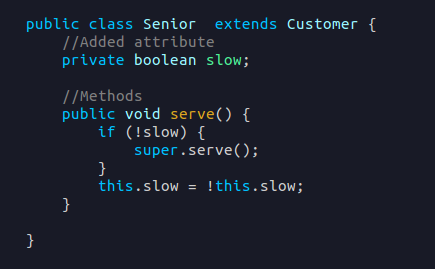
\includegraphics[width=15cm,height=6cm,keepaspectratio,]{Images/Senior}
  \caption{Senior class}
  \label{Figure 1.3}
\end{figure}


 In Figure 3\footnote{van den Eijkhof, Joy E, and Ulf Sigvardsson. 2 Nov. 2017. Came up with the logic behind Serve().} the subclass Senior has been created with its own added attribute and its own serve-method, overriding the Superclass’ Customers serve() method. By doing this, there are three points of SoC that can be pointed out from the above example:
\begin{enumerate}
\item The Senior Class can override all Customer Methods so that it suits the class, rather than editing in every Customer method, to take the isASenior attribute from Figure 1.2 into consideration. 
\item The Senior class serve method still refers back to the Super class’s serve method, which means that if that method were to be changed, it would not have to be changed in two places, but only in one, which is the benefit of non-repetitiveness.  
\item If a new type of Customer was to be introduced, then rather than introducing a new attribute such as isAFamily, one could instead add another subclass to Customers, which means the program is more developer friendly.
\end{enumerate}


\section{The impossible ideal}
The scientist Edsger W.Dijkstra who coined the term “Seperation of Concerns” said that “...even if not perfectly possible, [Seperation of Concerns] is yet the only available technique for effective ordering of one's thoughts, that I know of” \footnote{Dijkstra, Edsger W. “On the Role of Scientific Thought.” 30 Aug. 1974, NUENEN, The Netherlands.}  Is SoC really achievable? It is, as above examples have illustrated, but as Edsger W.Dijkstra pointed out, it is not perfectly possible. By the very nature of a program, that functions call upon functions, and methods call upon methods, true separation can never truly be achieved. This challenge can be considered in cross cutting concerns, concerns that are applicable to a whole complex, and affects the whole complex, and therefore cannot be properly encapsulated. Aspect Oriented Programming (AOP) languages try to address this issue by introducing something called an Advice. An Advice is code that is executed when different types of joint-points, such as when a method calls or receives data , is happened upon. AOP is able encapsulate joint points and change the way the code is run.\footnote{Pollice, Gary. “Aspect-Oriented Programming: What Is It Good for?” IBM- United States, Developerworks, 15 Mar. 2006, www.ibm.com/developerworks/rational/library/mar06/pollice/index.html.}  However, AOP falls short of the ideal as well, as the isolation of concerns can still be broken. 

\section{Conclusion}
Separation of Concerns (SoC) means to write a program in such a way that all its pieces deal with one coherent problem at a time. It is a worthwhile design principle to uphold as it keeps order, and that order maintains coherency and easier maintainability of a program. Although the ideal SOC cannot be achieved, it is still a worthwhile pursuit. Apply SoC, for remember, the code of a program in use is never done, but always under construction. 

\section{Sources}
\begin{enumerate}
\item Makabee, Hayim. “Separation of Concerns.” \textit{Effective Software Design}, 5 Feb. 2012, effectivesoftwaredesign.com/2012/02/05/separation-of-concerns/.
\item  Dijkstra, Edsger W. “On the Role of Scientific Thought.” 30 Aug. 1974, NUENEN, The Netherlands.
\item Pollice, Gary. “Aspect-Oriented Programming: What Is It Good for?” IBM - United States, Developerworks, 15 Mar. 2006, www.ibm.com/developerworks/rational/library/mar06/pollice/index.html.
\item van den Eijkhof, Joy E, and Ulf Sigvardsson. 2 Nov. 2017. Came up with the logic behind Serve().
\end{enumerate}

\end{flushleft}
\end{document}



